\documentclass[11pt,a4paper]{article}

\usepackage[indonesian]{babel}
\usepackage{fontspec}
\setmainfont{Times New Roman}
\setsansfont{Arial}
\setmonofont{Consolas}[Scale=0.88]

\usepackage[top=2.4cm,bottom=2.2cm,left=2.5cm,right=2.3cm,headheight=14pt]{geometry}
\usepackage{graphicx}
\usepackage{xcolor}
\usepackage{titlesec}
\usepackage{fancyhdr}
\usepackage{lastpage}
\usepackage{tabularx}
\usepackage{array}
\usepackage{colortbl}
\usepackage{enumitem}
\usepackage{setspace}
\usepackage{parskip}
\usepackage{needspace}
\usepackage{tikz}
\usetikzlibrary{arrows.meta,positioning,shapes.geometric}
\usepackage{listings}
\usepackage{hyperref}

\definecolor{PolibatamBlue}{HTML}{2F5496}
\definecolor{TableHeadBg}{HTML}{E8EEF6}
\definecolor{RowShade}{HTML}{F5F7FA}
\definecolor{JajanGreen}{HTML}{2E8B3D}
\definecolor{ActorFill}{HTML}{F0F6FC}

\lstset{
  basicstyle=\ttfamily\fontsize{8.5}{10.5}\selectfont,
  backgroundcolor=\color{RowShade},
  frame=single,
  rulecolor=\color{PolibatamBlue},
  breaklines=true,
  columns=fullflexible,
  keepspaces=true,
  showstringspaces=false,
  commentstyle=\color{JajanGreen}\itshape,
  keywordstyle=\color{PolibatamBlue}\bfseries,
  stringstyle=\color{black!75}
}

\hypersetup{
  colorlinks=true,
  linkcolor=PolibatamBlue,
  urlcolor=PolibatamBlue,
  pdftitle={Dokumentasi Audit Kode Fitur F008 dan F009 - JajanRia}
}

\titleformat{\section}
  {\normalfont\fontsize{13}{16}\bfseries}
  {\textcolor{PolibatamBlue}{\thesection.}}
  {0.6em}
  {}
\titleformat{\subsection}
  {\normalfont\fontsize{11.5}{14}\bfseries}
  {\textcolor{PolibatamBlue}{\thesubsection}}
  {0.6em}
  {}

\titlespacing*{\section}{0pt}{11pt}{5pt}
\titlespacing*{\subsection}{0pt}{8pt}{3pt}

\newcolumntype{L}[1]{>{\raggedright\arraybackslash}p{#1}}
\newcolumntype{C}[1]{>{\centering\arraybackslash}p{#1}}
\newcolumntype{Y}{>{\raggedright\arraybackslash}X}

\fancypagestyle{plain}{%
  \fancyhf{}%
  \renewcommand{\headrulewidth}{0pt}%
  \renewcommand{\footrulewidth}{0pt}%
  \fancyfoot[C]{%
    \fontsize{9}{11}\selectfont\sffamily
    \begin{tabular*}{\textwidth}{@{}l@{\extracolsep{\fill}}c@{\extracolsep{\fill}}r@{}}
      Dokumentasi Audit Kode JajanRia (PBL-TRPL104) & Fitur F008 \& F009 & Halaman \thepage{} dari \pageref{LastPage}
    \end{tabular*}%
  }%
}
\pagestyle{plain}

\begin{document}
\setstretch{1.15}
\emergencystretch=2em

% === HEADER DOKUMEN ===
\noindent
\begin{tabularx}{\textwidth}{@{}C{2.0cm}Y@{}}
  \raisebox{-0.45\height}{
\includegraphics[width=1.7cm]{assets/polibatam_logo.png}} &
  {\sffamily\bfseries\fontsize{14.5}{18}\selectfont\color{PolibatamBlue} Dokumentasi Teknis \& Audit Kode Fitur F008 dan F009}\\[3pt]
  & {\sffamily\small Platform E-Commerce Kuliner Kampus \textbf{JajanRia} (Semi-Automated Direct Commerce)}\\
  & {\sffamily\footnotesize Fokus Audit: Verifikasi Pembayaran (Admin \& Seller), Pengelolaan Pesanan, \& Pengamanan Akses \textbullet{} 24 November 2026}
\end{tabularx}
\vspace{0.15cm}
{\color{JajanGreen}\hrule height 1.5pt}
\vspace{0.3cm}

\section{Peta Spesifikasi, Rute, dan Otorisasi (F008 \& F009)}

Fitur \textbf{F008} dan \textbf{F009} mengatur tahap verifikasi pembayaran manual hingga penyelesaian pesanan \textit{Self Pick-up} sebelum sistem memicu tombol ulasan pembeli (\textbf{F010}). Untuk kelancaran operasional toko di luar jam kerja Administrator, verifikasi pembayaran (\textbf{F008}) kini dapat dilakukan oleh \textbf{Administrator} maupun \textbf{Seller} khusus pada pesanan lapaknya sendiri.

\renewcommand{\arraystretch}{1.22}
\begin{tabularx}{\textwidth}{|C{1.1cm}|L{3.1cm}|L{3.9cm}|Y|}
\hline
\rowcolor{TableHeadBg}
\textbf{Kode} & \textbf{Lingkup Fungsional} & \textbf{Rute \& \textit{Middleware}} & \textbf{Kontroler \& Berkas Antarmuka} \\
\hline
\textbf{F008} & Verifikasi bukti bayar (\textit{lunas} / \textit{ditolak} + alasan) oleh Admin dan Seller pemilik lapak. & \texttt{POST /admin/payments/\allowbreak \{id\}/verify} (\texttt{role:admin}); \texttt{POST /seller/orders/\allowbreak \{id\}/verify-payment} (\texttt{role:seller}) & \texttt{AdminController::\allowbreak verifyPayment}, \texttt{SellerController::\allowbreak verifyPayment}; \texttt{admin/dashboard.blade.php}, \texttt{seller/dashboard.blade.php}, \texttt{public/js/seller.js} \\
\hline
\textbf{F009} & Tampilan rincian item (\texttt{items\_detail}), \texttt{catatan\_pembeli}, status bayar, dan penyelesaian pesanan (\textit{selesai}) khusus pesanan \textit{lunas}. & \texttt{GET /seller?tab=orders}; \texttt{POST /seller/orders/\allowbreak \{id\}/status} (\texttt{role:seller}) & \texttt{SellerController::index}, \texttt{SellerController::\allowbreak updateOrderStatus}; \texttt{seller/dashboard.blade.php} \\
\hline
\end{tabularx}

\section{Diagram Workflow End-to-End F008 dan F009}

Gambar~\ref{fig:wf-f008-f009} menjelaskan alur transisi status pada tabel \texttt{t\_pesanan} mulai dari bukti bayar menunggu verifikasi hingga pesanan diselesaikan.

\begin{figure}[htbp]
\centering
\resizebox{\textwidth}{!}{%
\begin{tikzpicture}[
  box/.style={draw=PolibatamBlue, thick, rounded corners=3pt, fill=ActorFill, minimum width=3.1cm, minimum height=1.0cm, align=center, font=\sffamily\scriptsize, inner sep=4pt},
  srv/.style={draw=JajanGreen, thick, rounded corners=3pt, fill=green!6, minimum width=3.2cm, minimum height=1.0cm, align=center, font=\sffamily\scriptsize, inner sep=4pt},
  err/.style={draw=red!70!black, thick, rounded corners=3pt, fill=red!6, minimum width=2.8cm, minimum height=0.9cm, align=center, font=\sffamily\scriptsize, inner sep=4pt},
  arr/.style={->, >=Stealth, thick, PolibatamBlue},
  earr/.style={->, >=Stealth, thick, red!70!black},
  lbl/.style={font=\sffamily\tiny\bfseries, fill=white, inner sep=1pt}
]
  \node[box] (in) at (0, 0) {\textbf{1. Bukti Masuk (F007)}\\Status: \texttt{menunggu\_verifikasi}\\Status pesanan: \texttt{diproses}};
  \node[srv] (ver) at (4.6, 0) {\textbf{2. Verifikasi Bayar (F008)}\\Admin (\texttt{/admin}) atau\\Seller pemilik lapak (\texttt{/seller})};
  \node[err] (rej) at (9.3, 0) {\textbf{3a. Ditolak (\texttt{ditolak})}\\Simpan \texttt{catatan\_admin};\\Pembeli unggah ulang struk};

  \node[srv] (lunas) at (4.6, -2.35) {\textbf{3b. Disetujui (\texttt{lunas})}\\Reset \texttt{catatan\_admin=null};\\Tombol ``Selesai'' Seller aktif};
  \node[box] (prep) at (0, -2.35) {\textbf{4. Siapkan Self Pick-up}\\Seller cek \texttt{items\_detail}\\dan \texttt{catatan\_pembeli}};
  \node[srv] (fin) at (0, -4.65) {\textbf{5. Klik Selesai (F009)}\\Cek \texttt{status\_pembayaran==lunas},\\set \texttt{status=selesai}};
  \node[err] (blk) at (4.6, -4.65) {\textbf{Blokir Jika Belum Lunas}\\Tolak perubahan status\\(\textit{redirect} + pesan galat)};
  \node[box] (rev) at (9.3, -4.65) {\textbf{6. Pemicu Ulasan (F010)}\\Catat \texttt{waktu\_selesai};\\Tombol ``Beri Penilaian'' aktif};

  \draw[arr] (in) -- node[lbl, above] {Cek struk} (ver);
  \draw[earr] (ver) -- node[lbl, above] {Tolak} (rej);
  \draw[arr] (ver.south) -- node[lbl, right] {Setujui} (lunas.north);
  \draw[arr] (lunas.west) -- node[lbl, above] {Proses} (prep.east);
  \draw[arr] (prep.south) -- node[lbl, left] {Diambil} (fin.north);
  \draw[earr] (fin.east) -- node[lbl, above] {Belum lunas} (blk.west);
  \draw[arr] (fin.south) -- (0, -5.55) -| node[lbl, above, pos=0.25] {Lolos validasi lunas} (rev.south);
\end{tikzpicture}%
}
\caption{Diagram \textit{Workflow} Verifikasi Pembayaran (F008) dan Penyelesaian Pesanan (F009)}
\label{fig:wf-f008-f009}
\end{figure}

\section{Bedah Kode Backend \& Keamanan (Audit Dosen)}

\subsection{Lapisan Middleware (\texttt{app/Http/Middleware/EnsureRole.php})}
Seluruh rute F008 dan F009 dilindungi oleh \textit{middleware} \texttt{role:admin} atau \texttt{role:seller} (\texttt{EnsureRole::handle}, baris 15--49):
\begin{enumerate}[leftmargin=1.5em, itemsep=2pt, topsep=2pt]
  \item Memeriksa keberadaan sesi \texttt{session('user.id\_user')}; jika kosong, pengguna diarahkan ke \texttt{/login} (\texttt{HTTP 401} untuk permintaan JSON).
  \item Mengambil data terbaru dari \texttt{Pengguna::find(\$userId)} dan memastikan \texttt{\$user->is\_active == true}; akun nonaktif dihapus sesinya dan ditolak (\texttt{HTTP 403}).
  \item Khusus peran \texttt{seller}, memastikan \texttt{\$user->status\_\allowbreak verifikasi === 'terverifikasi'} sehingga Seller berstatus \textit{menunggu} atau \textit{ditolak} tidak dapat mengakses dasbor maupun memverifikasi transaksi.
  \item Mencocokkan \texttt{\$user->role === \$role}; akses lintas peran (misal Pengunjung mengakses rute Admin atau Seller) ditolak tegas dengan \texttt{abort(403)}.
\end{enumerate}

\subsection{Logika F008: Verifikasi Pembayaran oleh Admin \& Seller}
\begin{itemize}[leftmargin=1.5em, itemsep=2pt, topsep=2pt]
  \item \textbf{Admin (\texttt{AdminController::verifyPayment}, baris 259--277):} memvalidasi \texttt{status} (\texttt{required|in:lunas,ditolak}) dan \texttt{catatan} (\texttt{nullable|string|max:255}), memperbarui \texttt{status\_\allowbreak pembayaran} serta \texttt{catatan\_admin} pada \texttt{Pesanan::\allowbreak findOrFail(\$idPesanan)}, lalu kembali ke tab \texttt{payments}.
  \item \textbf{Seller (\texttt{SellerController::verifyPayment}, baris 248--274):} menerapkan validasi masukan yang sama, namun mengunci \textit{query} memakai \texttt{\$umkm = \$this->getSellerUmkm()} dan \texttt{Pesanan::where('id\_pesanan', \$id)->\allowbreak where('id\_umkm', \$umkm->id\_umkm)->\allowbreak firstOrFail()}. Dengan demikian, Seller hanya bisa memverifikasi pesanan lapaknya sendiri (percobaan lintas lapak menghasilkan \texttt{HTTP 404}). Jika disetujui \texttt{lunas}, \texttt{catatan\_admin} otomatis direset menjadi \texttt{null}.
\end{itemize}

\needspace{6.5cm}
\begin{lstlisting}[language=PHP,caption={Isolasi Kepemilikan UMKM pada \texttt{SellerController::verifyPayment} (F008)}]
$umkm = $this->getSellerUmkm();
$pesanan = Pesanan::where('id_pesanan', $id)
    ->where('id_umkm', $umkm->id_umkm)
    ->firstOrFail(); // Menolak akses lintas lapak (HTTP 404)

$status = $request->input('status'); // 'lunas' atau 'ditolak'
$catatan = trim((string) $request->input('catatan'));

$pesanan->update([
    'status_pembayaran' => $status,
    'catatan_admin' => $status === 'lunas' ? null : ($catatan ?: null),
]);
\end{lstlisting}

\subsection{Logika F009: Daftar Pesanan \& Guard Penyelesaian (\texttt{SellerController})}
\begin{enumerate}[leftmargin=1.5em, itemsep=2pt, topsep=2pt]
  \item \textbf{Pengambilan Data (\texttt{SellerController::index}, baris 50--53):} mengambil pesanan milik lapak aktif saja (\texttt{Pesanan::where('id\_umkm', \$umkm->id\_umkm)->with(['pengunjung', 'umkm'])->latest()->get()}). Kolom JSON \texttt{items\_detail} otomatis ter-cast menjadi array oleh model \texttt{Pesanan}.
  \item \textbf{Guard Status Lunas (\texttt{SellerController::updateOrderStatus}, baris 220--243):} memvalidasi \texttt{status} (\texttt{required|in:diproses,selesai}), mengecek kepemilikan \texttt{id\_umkm}, dan menegakkan aturan bisnis keras agar pesanan belum lunas tidak dapat diselesaikan.
  \item \textbf{Persistensi Tab (\texttt{redirectToTab}):} setiap aksi POST mengarahkan kembali ke \texttt{route('seller', ['tab' => 'orders'])} sehingga Seller tidak terlempar ke tab awal.
\end{enumerate}

\begin{lstlisting}[language=PHP,caption={Guard Status Lunas pada \texttt{SellerController::updateOrderStatus} (F009)}]
if ($status === 'selesai' && $pesanan->status_pembayaran !== 'lunas') {
    return $this->redirectToTab($request, 'orders')
        ->with('error', 'Pesanan #' . $id . ' belum dapat diselesaikan karena pembayaran belum diverifikasi LUNAS.');
}
$pesanan->update([
    'status' => $status,
    'waktu_selesai' => $status === 'selesai' ? Carbon::now() : null,
]);
\end{lstlisting}

\section{Bedah Kode Frontend (Blade \& Vanilla JS)}

\begin{enumerate}[leftmargin=1.5em, itemsep=2pt, topsep=2pt]
  \item \textbf{Panel Administrator (\texttt{admin/dashboard.blade.php}, baris 610--626 \& 1203--1249):} tab \texttt{payments} merender pratinjau struk, tombol formulir ``Setujui'' (\texttt{status=lunas}), serta tombol ``Tolak'' yang memanggil \texttt{openRejectPaymentModal(id)} untuk mengisi \texttt{action} formulir modal \texttt{\#rejectPaymentModalBackdrop} dengan alasan penolakan.
  \item \textbf{Dasbor Seller (\texttt{seller/dashboard.blade.php}, baris 500--571 \& 881--910):} pada tab \texttt{orders}, tiap baris menampilkan daftar \texttt{items\_detail}, \texttt{catatan\_pembeli}, tautan ``Lihat Struk'', dan lencana status pembayaran.
  \item \textbf{Kontrol Tombol Dinamis di Kolom Tindakan UMKM:}
    \begin{itemize}[leftmargin=1.2em, itemsep=1pt]
      \item Jika \texttt{status\_pembayaran === 'lunas'} dan \texttt{status === 'diproses'}: tampil tombol ``Selesai'' (\texttt{route('seller.orders.status')}).
      \item Jika \texttt{status\_pembayaran === 'menunggu\_verifikasi'} atau bukti foto sudah diunggah: tampil tombol ``Lunas'' (kirim langsung \texttt{status=lunas}) dan tombol ``Tolak'' (memanggil fungsi \texttt{openSellerReject\allowbreak PaymentModal(id)} di \texttt{public/js/seller.js}, membuka modal \texttt{\#sellerRejectPayment\allowbreak ModalBackdrop}).
    \end{itemize}
\end{enumerate}

\begin{figure}[htbp]
\centering
\begin{minipage}[t]{0.48\textwidth}
  \centering
  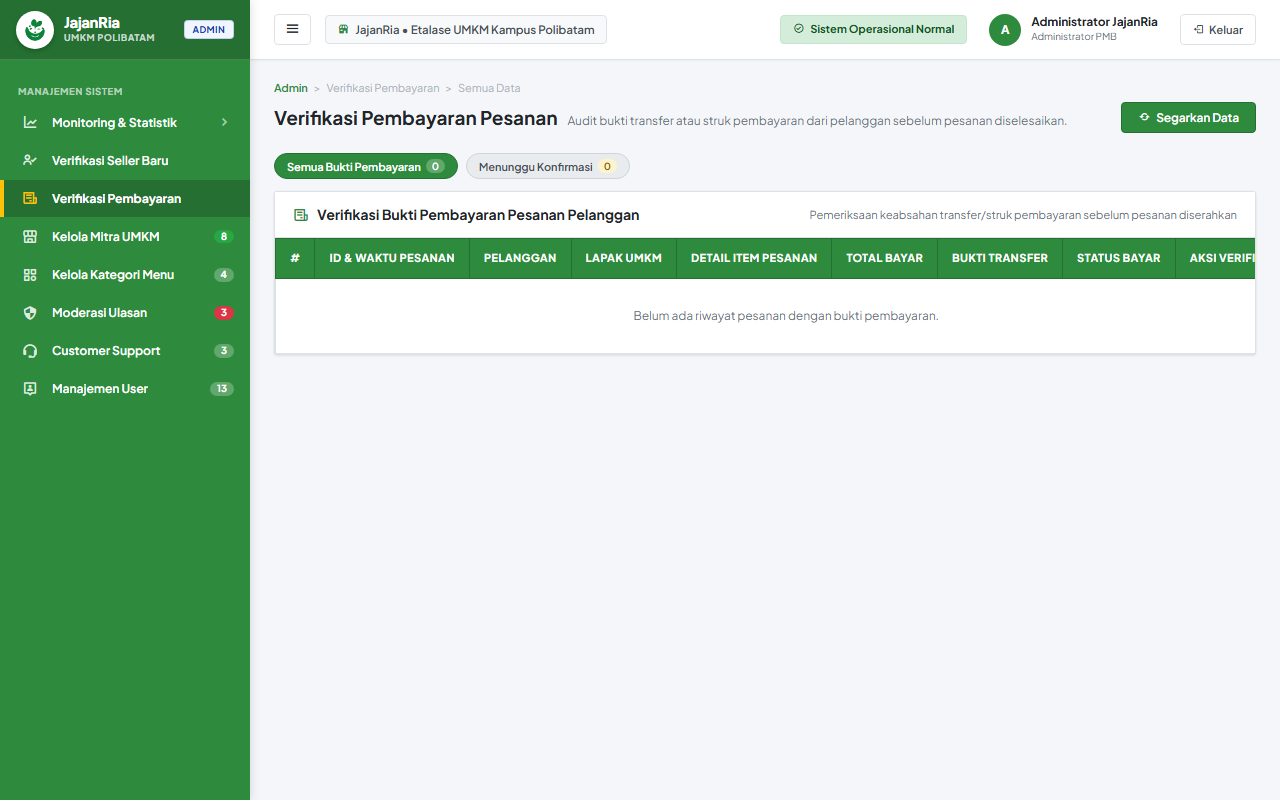
\includegraphics[width=\textwidth]{assets/screens/12_admin_payments.png}
  \par\small (a) Tab Verifikasi Pembayaran Admin (F008)
\end{minipage}\hfill
\begin{minipage}[t]{0.48\textwidth}
  \centering
  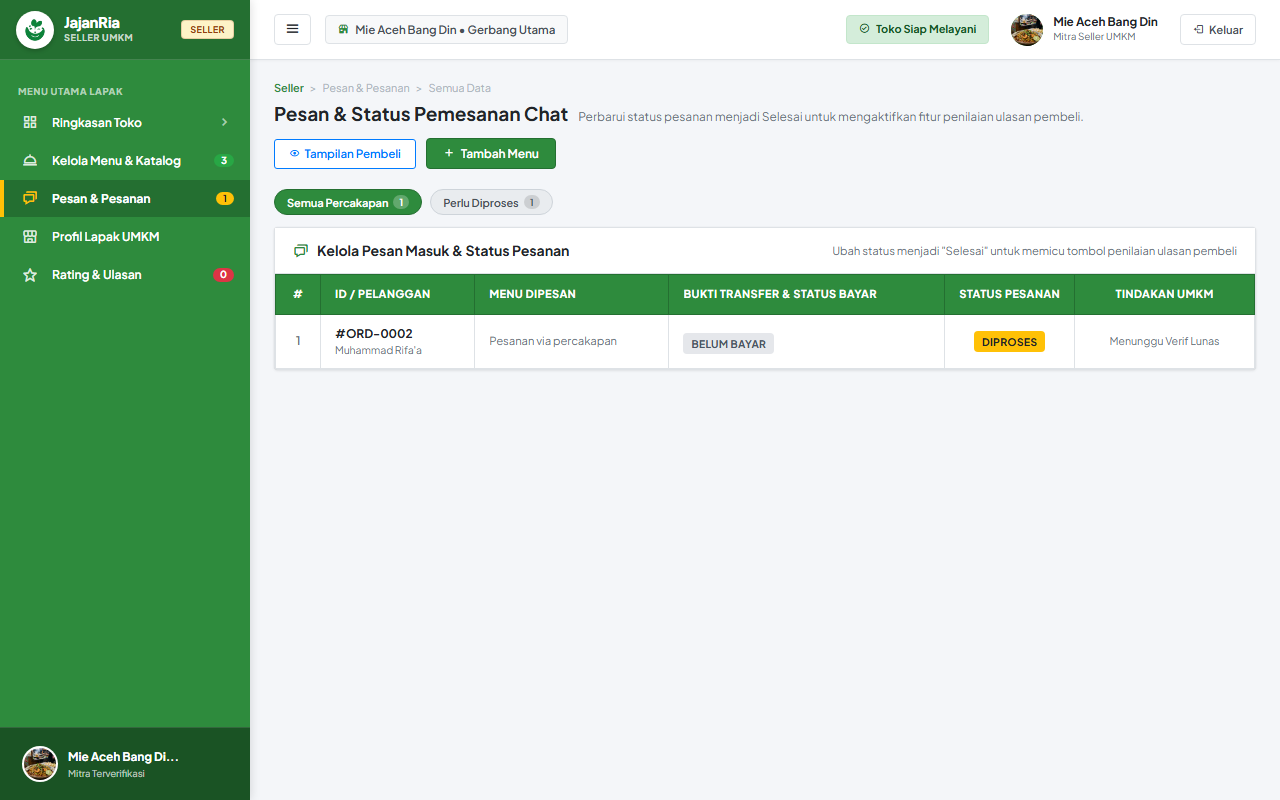
\includegraphics[width=\textwidth]{assets/screens/10_seller_orders.png}
  \par\small (b) Tab Pesan \& Pesanan Dasbor Seller (F008/F009)
\end{minipage}
\caption{Antarmuka Implementasi Verifikasi Pembayaran dan Pengelolaan Pesanan}
\label{fig:fe-f008-f009}
\end{figure}

\section{Checklist Tanya-Jawab Audit Dosen \& Hasil PHPUnit}

\renewcommand{\arraystretch}{1.20}
\begin{tabularx}{\textwidth}{|L{4.0cm}|Y|L{3.85cm}|}
\hline
\rowcolor{TableHeadBg}
\textbf{Pertanyaan Audit Dosen} & \textbf{Jawaban Teknis \& Penjelasan Kode} & \textbf{Lokasi Bukti Kode} \\
\hline
Bagaimana jika ada pihak memanggil endpoint \texttt{selesai} sebelum bayar? & Server menolak dengan pengecekan keras \texttt{status\_pembayaran !== 'lunas'} dan mengembalikan pesan galat; tombol UI juga disembunyikan. & \texttt{SellerController.php} baris 232--235 \\
\hline
Bagaimana mencegah Seller A memverifikasi/mengubah order Seller B? & Seluruh query pesanan memakai filter ganda \texttt{where('id\_umkm', \$umkm->id\_umkm)->firstOrFail()} berbasis sesi pemilik, menghasilkan \texttt{HTTP 404} jika lintas lapak. & \texttt{SellerController.php} baris 229, 259--261 \\
\hline
Bagaimana jika akun Pengunjung mencoba akses rute Admin/Seller? & \textit{Middleware} \texttt{EnsureRole} memvalidasi sesi, status aktif, dan kecocokan peran di setiap rute terproteksi, menolak akses dengan \texttt{HTTP 403}. & \texttt{EnsureRole.php} baris 15--49; \texttt{routes/web.php} \\
\hline
Mengapa Seller juga diizinkan memverifikasi pembayaran (F008)? & Agar transaksi toko tetap berjalan 24 jam tanpa bergantung pada Admin, dengan tetap mempertahankan isolasi per lapak dan Admin sebagai cadangan. & \texttt{SellerController::\allowbreak verifyPayment}; \texttt{AdminController::\allowbreak verifyPayment} \\
\hline
Bagaimana menjaga posisi halaman agar tidak reset ke awal? & Kontroler mengarahkan kembali melalui \texttt{redirectToTab(\$request, 'orders'/'payments')} dengan parameter query \texttt{tab} aktif. & \texttt{SellerController.php} baris 85--92 \\
\hline
\end{tabularx}

\vspace{0.25cm}
\noindent \textbf{Hasil Verifikasi PHPUnit (\texttt{php artisan test}):} seluruh skenario pada \texttt{F008F009\allowbreak OrderVerificationTest.php} dan \texttt{F006F007\allowbreak CheckoutTest.php} (total \textbf{9 pengujian, 37 asersi}) dinyatakan \textbf{LULUS (PASS)} dalam \textbf{1,44 detik}, meliputi persetujuan/penolakan Admin, verifikasi/isolasi Seller, pemblokiran penyelesaian sebelum lunas, penyelesaian setelah lunas dengan pencatatan \texttt{waktu\_selesai}, serta penolakan \texttt{HTTP 403} oleh \texttt{EnsureRole}.

\end{document}
